\titleformat{\section}[hang]
{\Large\bfseries}
{\thesection.}{0.4em}{}
\titlespacing{\section}{0pc}{0.5cm}{0.5cm}
\titleformat{\subsection}[hang]
{\large\bfseries}
{\thesubsection.}{0.4em}{}
\titlespacing{\subsection}{0pc}{0.4cm}{0.3cm}


\section{Expressiveness of logistic mixture coupling layers}
\label{sec:appendix_mixture_optimality}

The following section details the proof to show that under mild assumptions, Categorical Normalizing Flows with autoregressive logistic mixture coupling layers can be as powerful as other non-latent based recurrent neural networks with a pure autoregressive likelihood objective. 
This has not been the case for previous attempts on modeling categorical data with normalizing flows in continuous space as seen in \cite{SemiDiscreteNFSequence}.

We start with a single layer autoregressive mixture coupling layer and assume that the categories are encoded by a mixture of logistics. 
The base distribution is also a standard logistic.
Recall that the logistic mixture coupling for a single element $z$ is defined by the following transformation:
\begin{equation}
    y = \sigma^{-1}\left(\sum_{i=1}^{K} \pi_i \sigma\left(\frac{z-\mu_i}{\exp(-s_i)}\right)\right)\cdot \exp(a)+b
\end{equation}
where $\bm{\pi}, \bm{\mu}, \bm{\sigma}, a$ and $b$ are parameterized by a neural network, and $K$ is the number of mixtures.
As we are aiming to model a standard logistic as base distribution, we set $a=0,b=0$.
The log-determinant Jacobian (LDJ) of a mixture coupling layer for a single element is then as follows:
\begin{eqnarray}
\gamma_i & = & \frac{z-\mu_i}{\exp(-s_i)}\\
\text{LDJ}_{\text{coup}} & = & \log \left(\sum \pi_i \cdot \exp\left[\gamma_i - s_i - 2\log\left(1+\exp(\gamma_i)\right)\right]\right)\\
& = & \log \left(\sum \pi_i \cdot \exp\left[\gamma_i - s_i\right]/\left(1+\exp(\gamma_i)\right)^2\right)
\end{eqnarray}
The coupling layer maps a mixture of $K$ logistics back to a single one.
Hence, in this case, the optimal setting is if those $K$ mixtures represent the logistics for the categories in the encoding distribution.
Additionally, the variational framework ensures that we train the encoding mixtures to be clearly separated. 
Thus, we can assume that for a sampled latent $z$ from $q(z|x)$, $|\gamma_j|\gg0$ for all $j\in\{1,...,K\}$ except one, which we denote here with $i$. Then we can reduce the LDJ to:
\begin{eqnarray}
\text{LDJ}_{\text{coup}} & = & \log \pi_i + \gamma_i - s_i - 2\log\left(1+\exp(\gamma_i)\right)\\
& = & \log \pi_i + \log\left(\exp(\gamma_i)/\left(1+\exp(\gamma_i)\right)\right) - s_i - \log\left(1+\exp(\gamma_i)\right)\\
& = & \log \pi_i - s_i - \log\left(1+\exp(-\gamma_i)\right) - \log\left(1+\exp(\gamma_i)\right)
\end{eqnarray}	
Next, we have to add the LDJ we obtain from the encoding distribution. 
For a single element $z$, this is:
\begin{eqnarray}
\text{LDJ}_{\text{encode}} & = & s_i + \log\left(1+\exp(-\gamma_i)\right) + \log\left(1+\exp(\gamma_i)\right)
\end{eqnarray}
where we reuse the index $i$ from $\text{LDJ}_{\text{coup}}$. 
The overall objective we are left with for an input $x$ is:
\begin{eqnarray}
\text{LDJ}_{\text{model}} & = & \text{LDJ}_{\text{encode}} + \text{LDJ}_{\text{coup}} \\
& = & \log \pi_i
\end{eqnarray}	
Therefore, optimizing the logistic mixture coupling layer reduces to optimizing a softmax distribution over categories which is exactly the same objective as a standard autoregressive model on categorical distribution. 
We have shown that this property also holds in practice as can be seen at the experiments on language modeling (Section~\ref{sec:experiments_language_modeling}).

\newpage
\section{Visualization of the latent space}
\label{sec:appendix_latent_space_visualization}

In the following, we outline the visualization method of the latent space used in Section~\ref{sec:experiments_discussion_latent_space}.


\begin{figure}[b!]
    \centering
    \begin{tabular}{ccc}
        \textit{Encoding distribution} &
        \textit{Flow layer 1} & 
        \textit{Flow layer 2} \\
        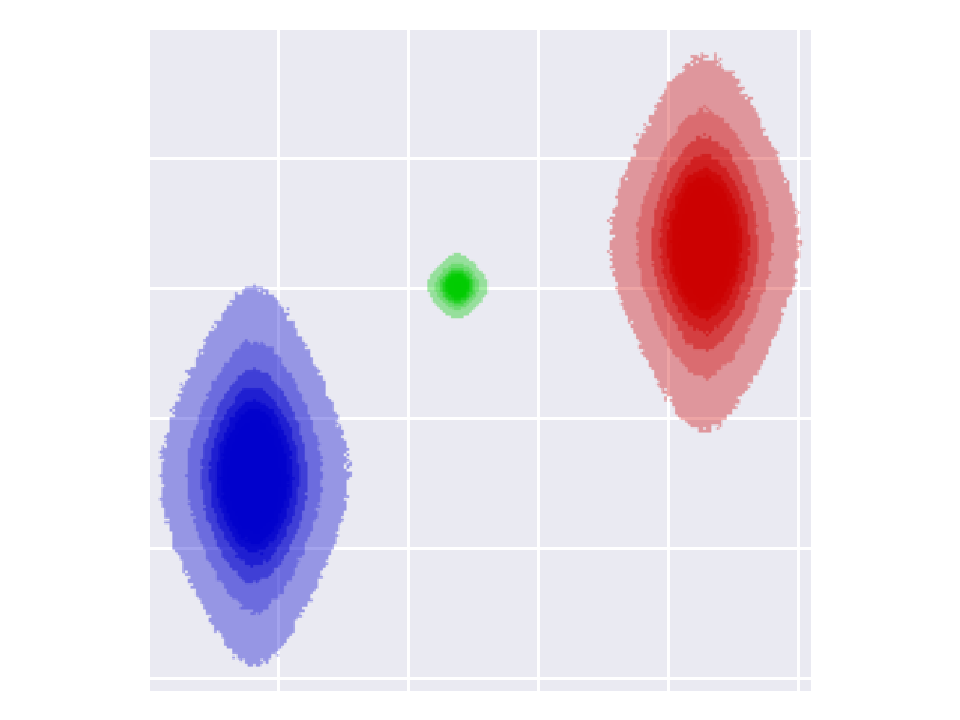
\includegraphics[width=0.3\textwidth]{figures/experiments_figures/latent_space/graph_coloring/layer_forward_01.pdf} & 
        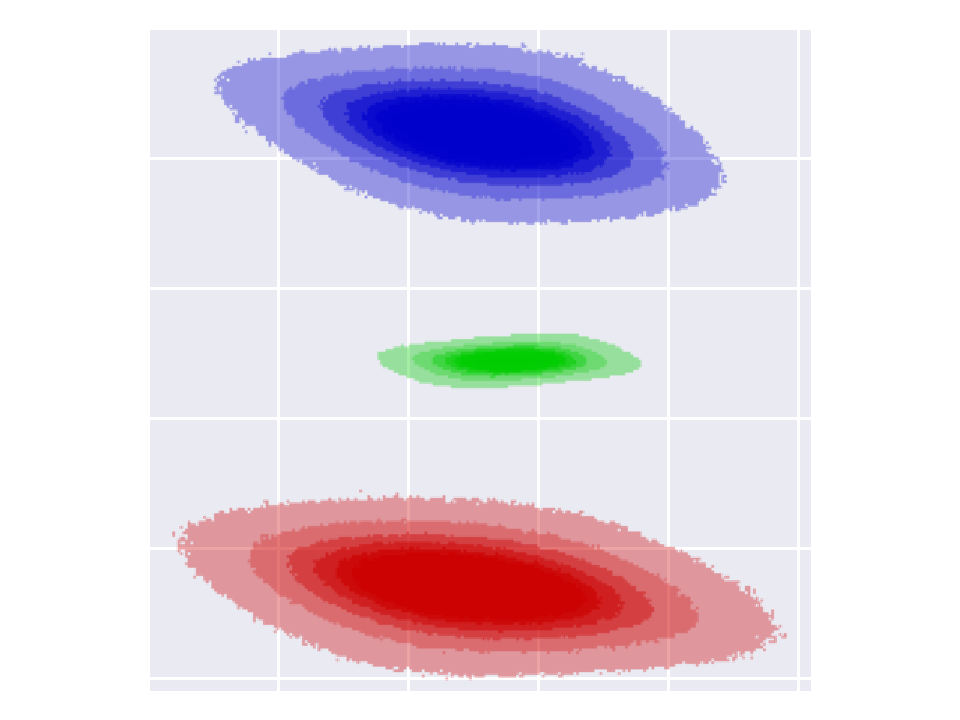
\includegraphics[width=0.3\textwidth]{figures/experiments_figures/latent_space/graph_coloring/layer_forward_04.pdf}  & 
        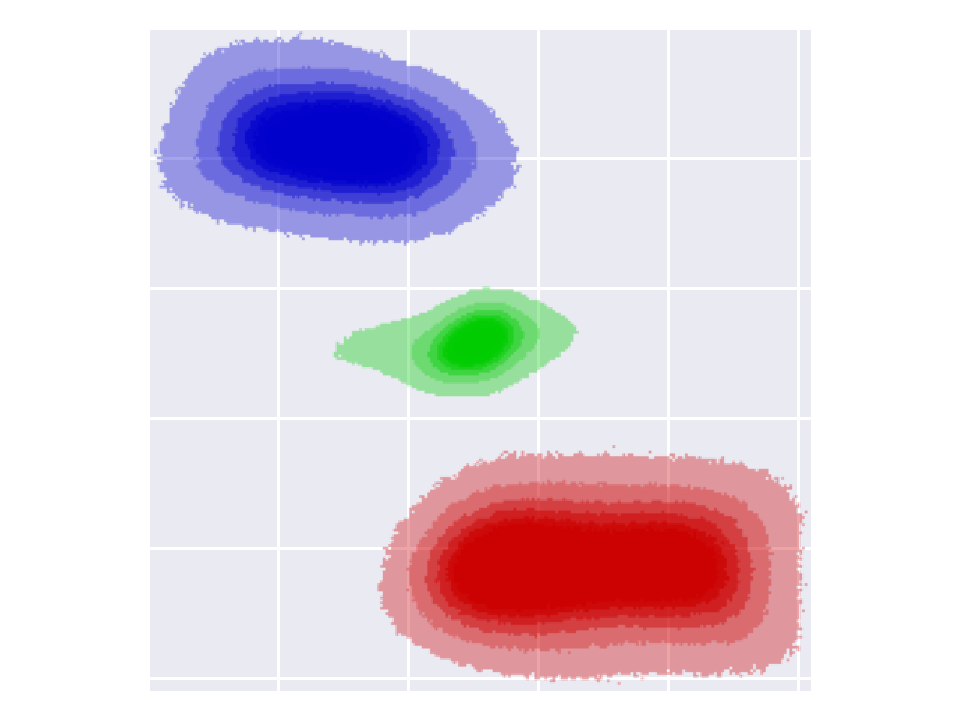
\includegraphics[width=0.3\textwidth]{figures/experiments_figures/latent_space/graph_coloring/layer_forward_07.pdf}
        \\[0.4cm]
        \textit{Flow layer 3} &
        \textit{Flow layer 4} & 
        \textit{Flow layer 5} \\
        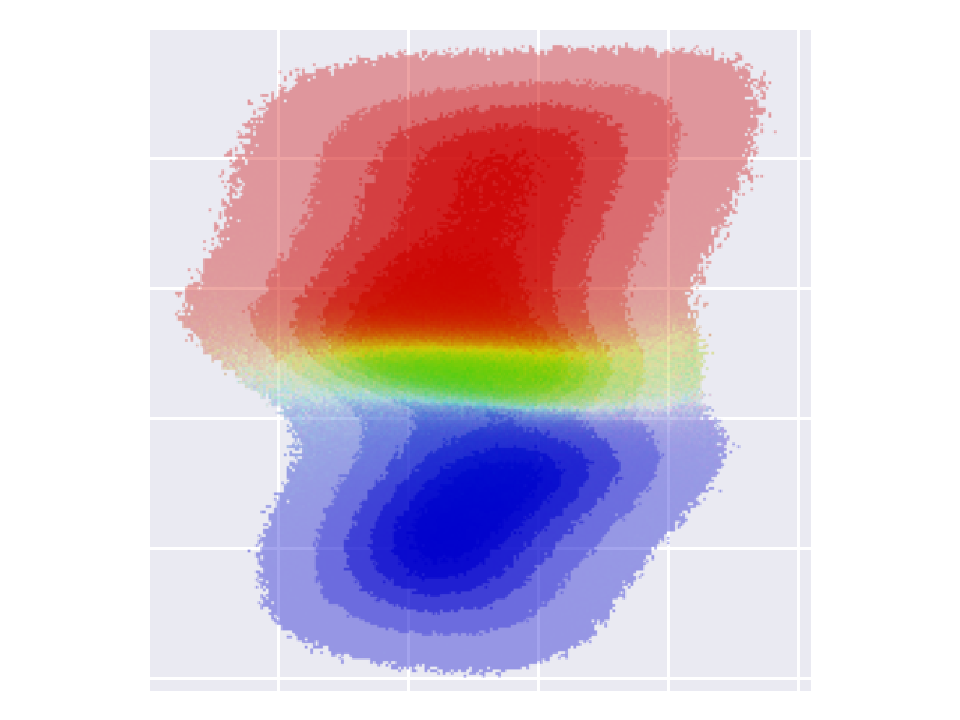
\includegraphics[width=0.3\textwidth]{figures/experiments_figures/latent_space/graph_coloring/layer_forward_10.pdf} & 
        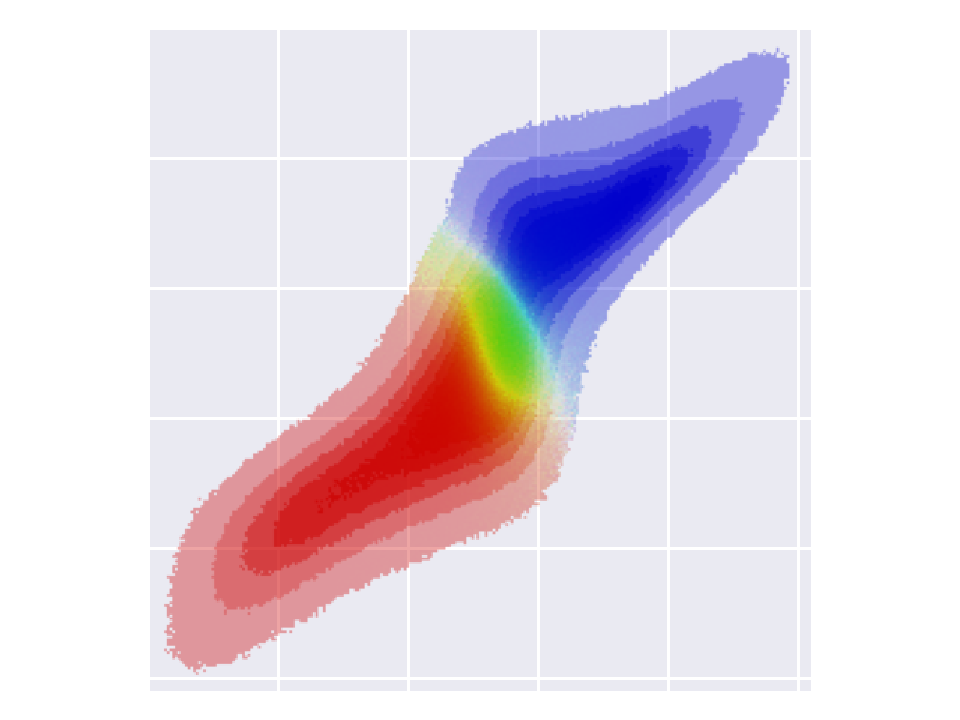
\includegraphics[width=0.3\textwidth]{figures/experiments_figures/latent_space/graph_coloring/layer_forward_13.pdf}  & 
        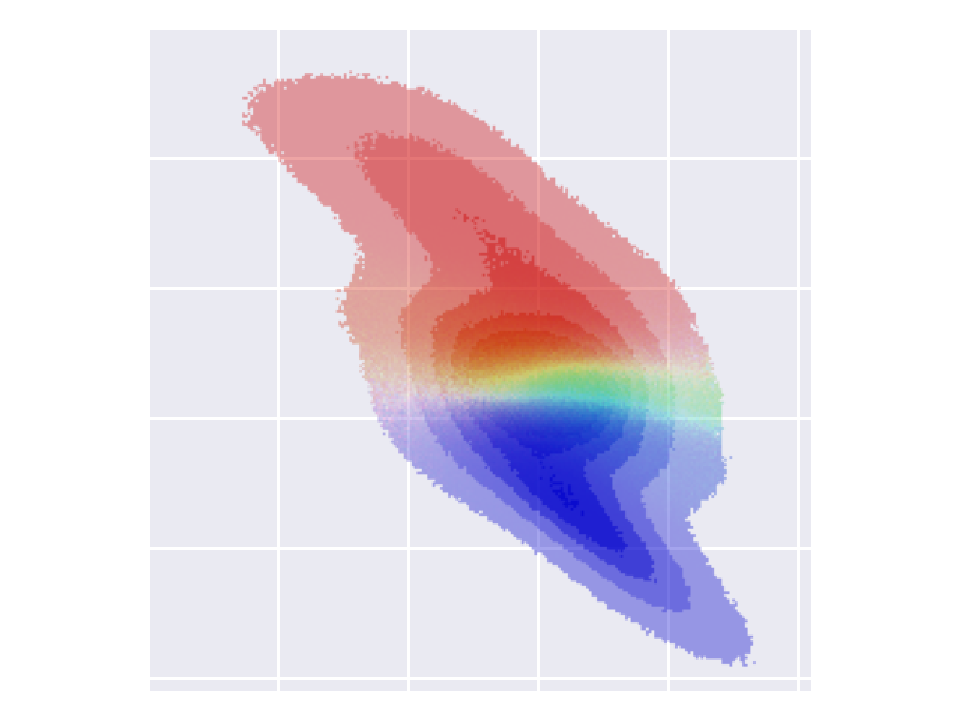
\includegraphics[width=0.3\textwidth]{figures/experiments_figures/latent_space/graph_coloring/layer_forward_16.pdf}
        \\[0.4cm]
        \textit{Flow layer 6} &
        \textit{Flow layer 7} & 
        \textit{Base distribution} \\
        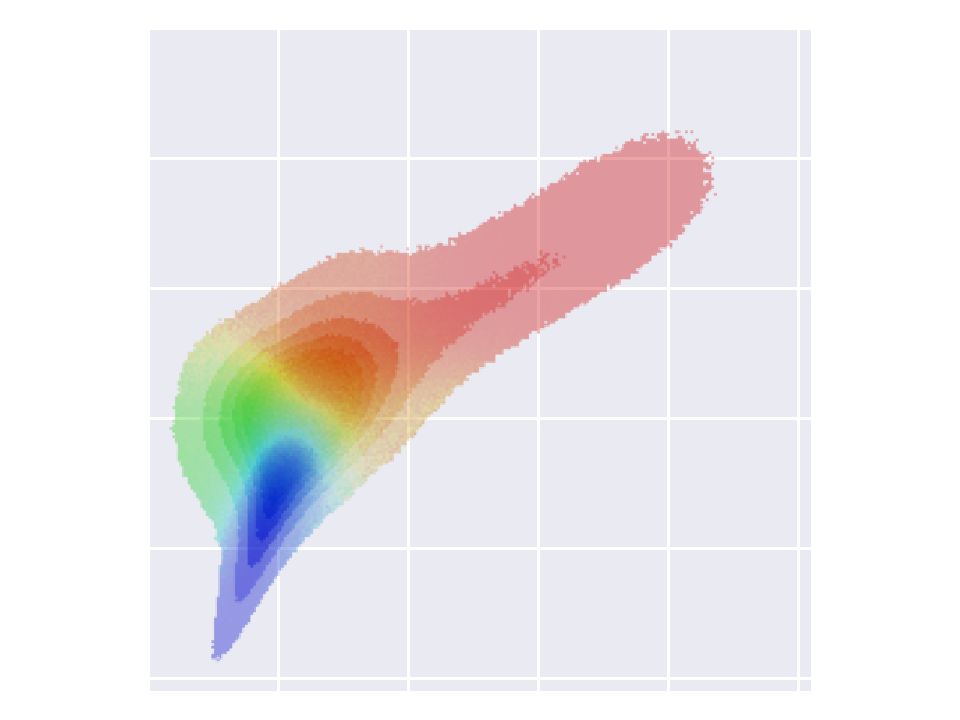
\includegraphics[width=0.3\textwidth]{figures/experiments_figures/latent_space/graph_coloring/layer_forward_19.pdf} & 
        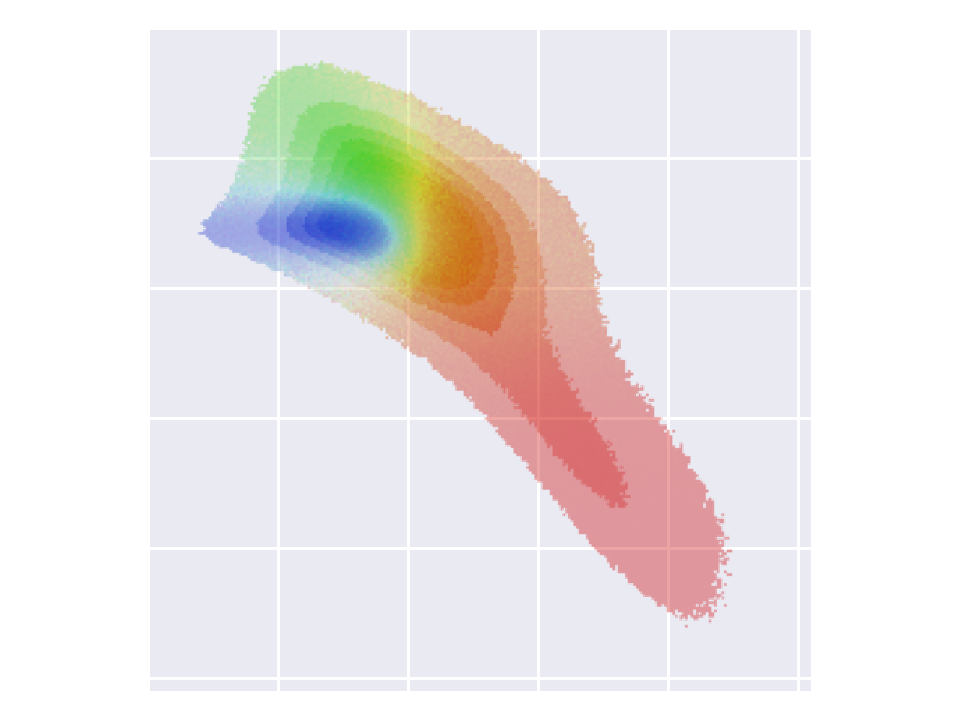
\includegraphics[width=0.3\textwidth]{figures/experiments_figures/latent_space/graph_coloring/layer_forward_22.pdf}  & 
        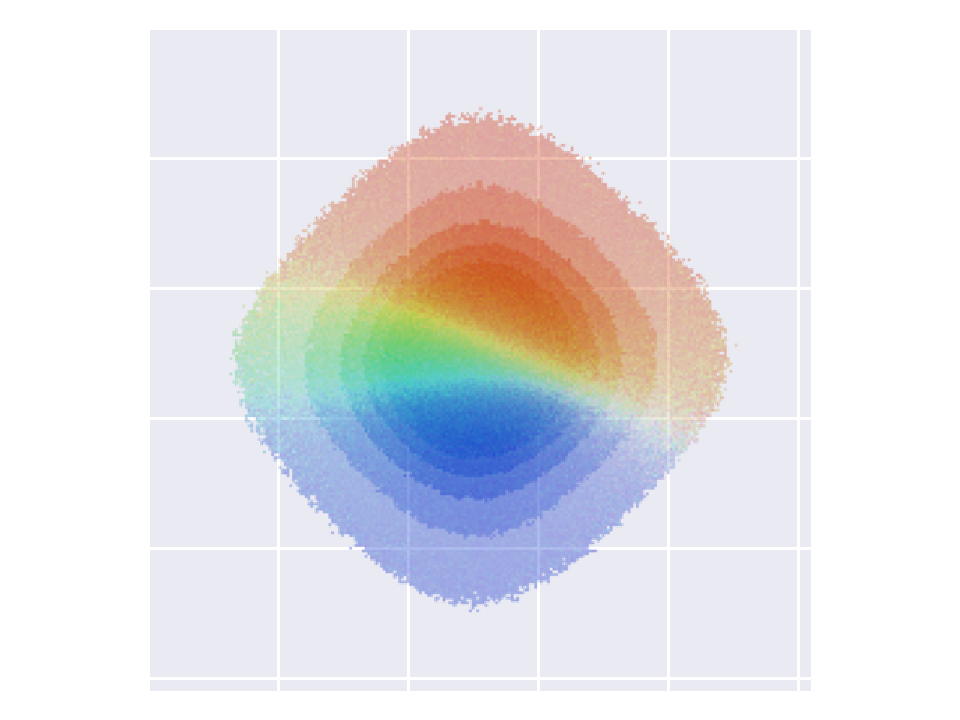
\includegraphics[width=0.3\textwidth]{figures/experiments_figures/latent_space/graph_coloring/layer_forward_25.pdf}
        \\
    \end{tabular}
    \caption[Complete latent space of graph coloring flow (large)]{Visualization of the latent space for all 8 layers of the flow applied on graph coloring (see Figure~\ref{fig:experiments_discussion_latent_space_graph_coloring} for an explanation of the figure). We only show the forward direction as the reverse only differs in negligible aspects.}
    \label{fig:appendix_latent_space_visualization_graph_coloring}
\end{figure}

The first step we take is to collect about 8,000 examples from the training set and forward them through the model as we have done it during training.
Thereby, we save the latent representation $\bm{z}$ after each flow block consisting of an activation normalization, invertible 1x1 convolutions, and a logistic mixture coupling layer.
To reduce the variance, we repeat this process 32 times, each time with different samples from the encoding distribution $q(\bm{z}|\bm{x})$.
After collecting all samples, we convert the observed latents per layer into a histogram in the continuous space with 512 bins for each dimension.
Additionally, we accumulate the histograms across categorical variables to obtain a more stable and general impression of the probability densities in latent space.

To show the densities per category, we color the bins depending on the proportion of latents that represent a specific category. 
For instance, for graph coloring, we visualize the three categories with blue, green, and red. 
If at a position multiple categories occur, we average their RGB color based on the proportion of latents assigned to each category.
In order to see the latent space of all categories equally, we normalize the probability density per category independently.
This means that we first create a histogram for each category separately, then normalize it to have a maximum of 1, and finally combine the histogram of all categories.
Although this strategy does not represent densities across categories correctly, we are able to visualize the densities per category accurately and have no issues with strongly peaked distribution.
If we would have normalized the joint histogram, for instance, the blue and red densities in the encoding distribution (Figure~\ref{fig:appendix_latent_space_visualization_graph_coloring}) would not have been visible.

Finally, we also bin the histogram values to get a clearer distinction between dense and sparse probability mass.
Areas with lower density are more transparent than other parts in the figure and appear with a lighter color.
This gives us finally latent space visualization shown in Figure~\ref{fig:experiments_discussion_latent_space_graph_coloring}, \ref{fig:experiments_discussion_latent_space_set} and \ref{fig:appendix_latent_space_visualization_graph_coloring}.

% \begin{figure}[b!]
%     \centering
%     \begin{tabular}{ccc}
%         \textit{Encoding distribution} &
%         \textit{Flow layer 1} & 
%         \textit{Flow layer 2} \\
%         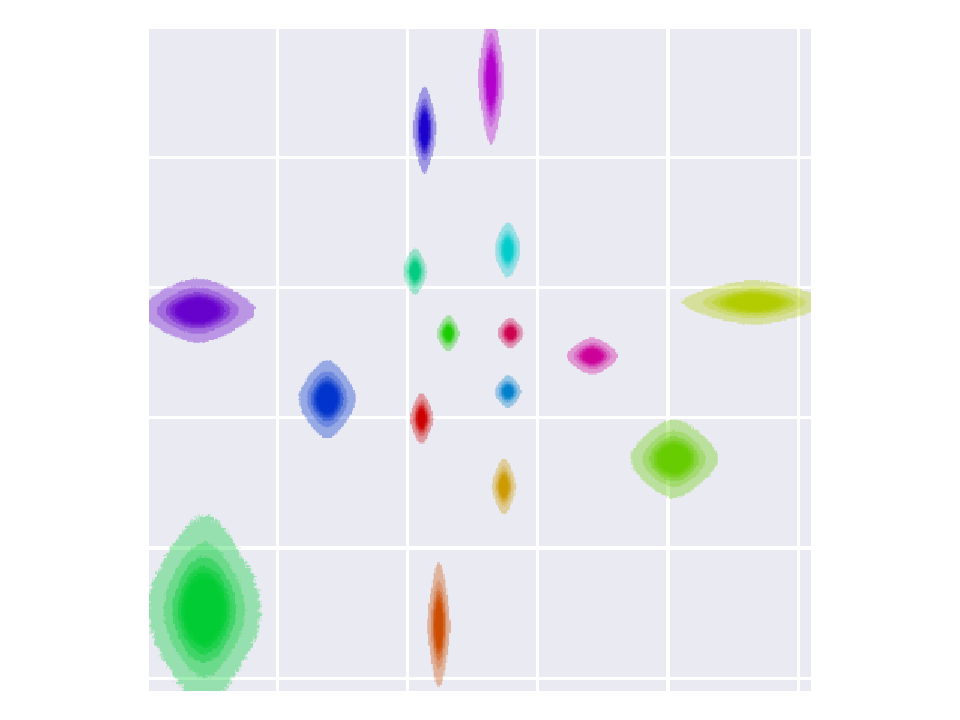
\includegraphics[width=0.3\textwidth]{figures/experiments_figures/latent_space/set_modeling/layer_forward_01.pdf} & 
%         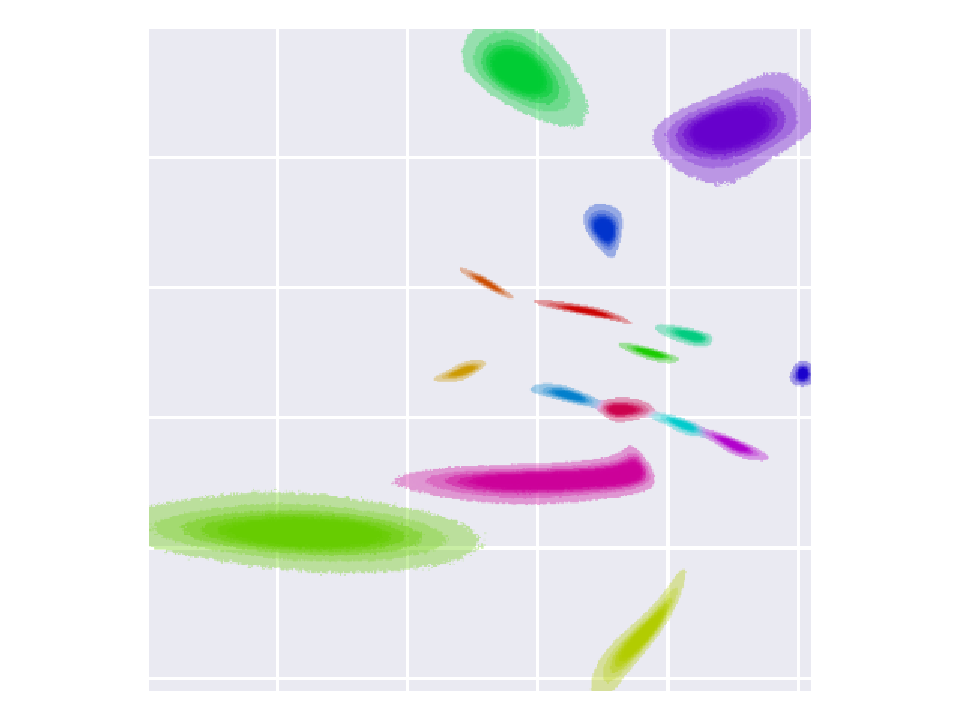
\includegraphics[width=0.3\textwidth]{figures/experiments_figures/latent_space/set_modeling/layer_forward_04.pdf} & 
%         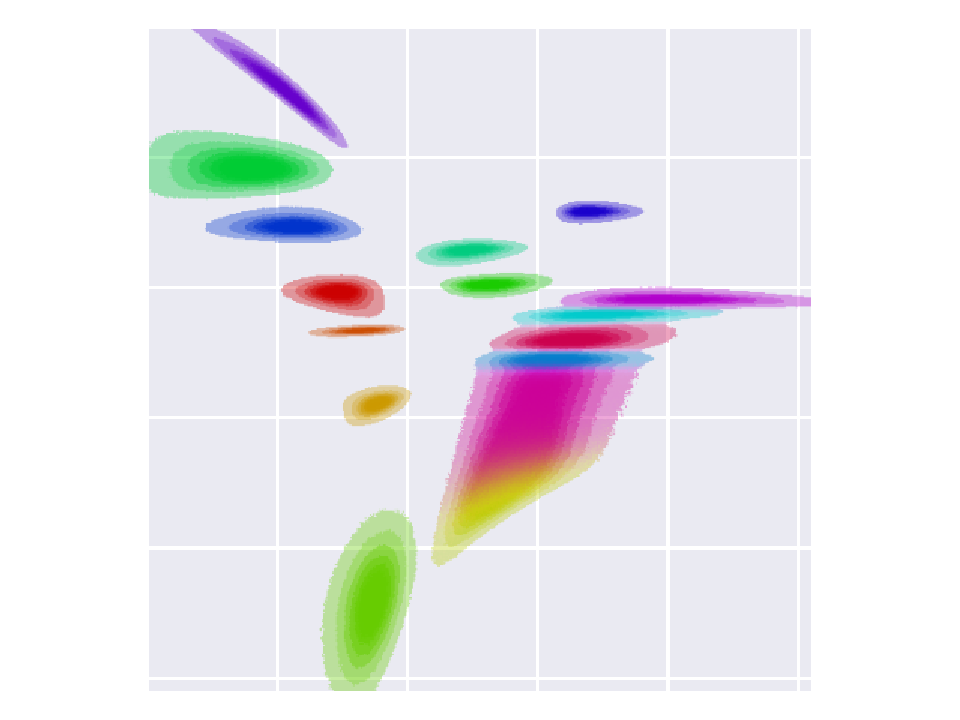
\includegraphics[width=0.3\textwidth]{figures/experiments_figures/latent_space/set_modeling/layer_forward_07.pdf}
%         \\[0.4cm]
%         \textit{Flow layer 3} &
%         \textit{Base distribution} & \\
%         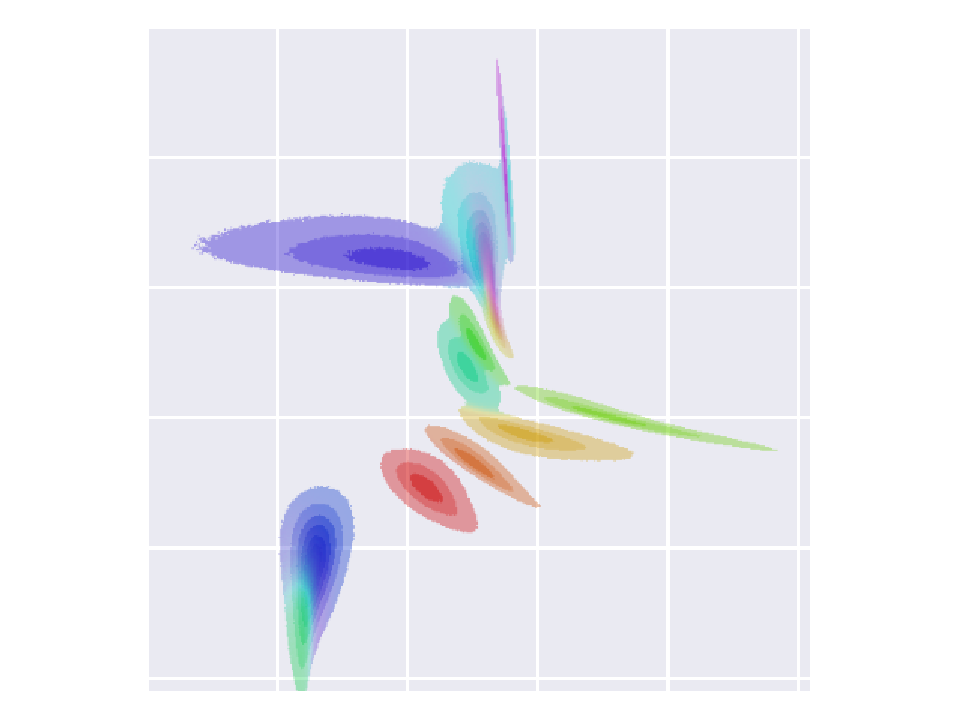
\includegraphics[width=0.3\textwidth]{figures/experiments_figures/latent_space/set_modeling/layer_forward_10.pdf} & 
%         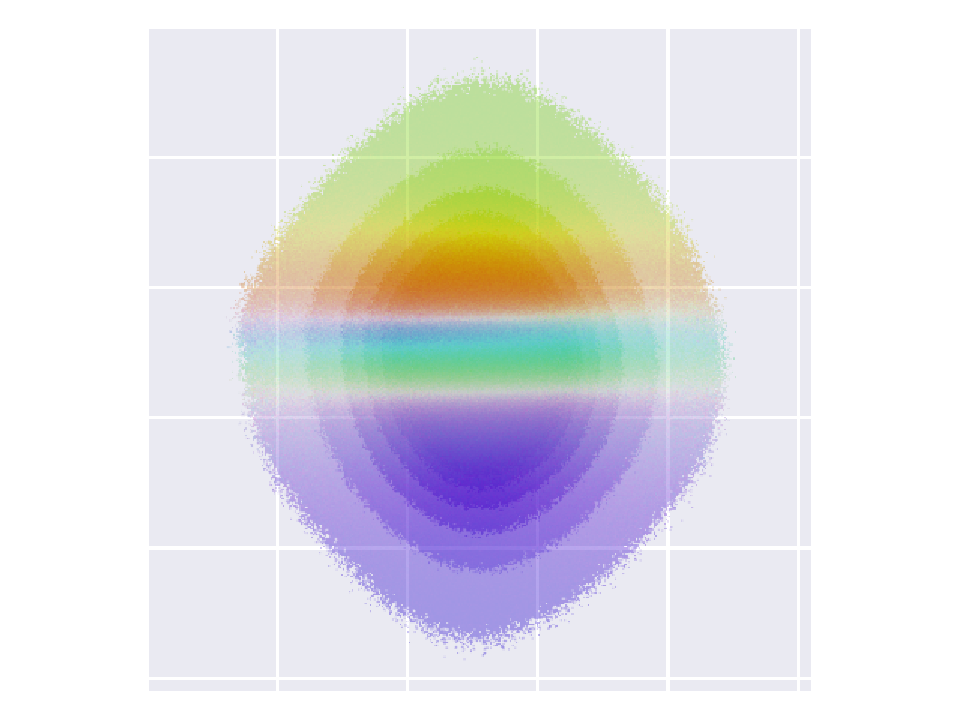
\includegraphics[width=0.3\textwidth]{figures/experiments_figures/latent_space/set_modeling/layer_forward_13.pdf} & 
%         \\
%     \end{tabular}
%     \caption[Complete latent space of graph coloring flow (large)]{Visualization of the latent space for all 8 layers of the flow applied on graph coloring (see Figure~\ref{fig:experiments_discussion_latent_space_graph_coloring} for an explanation of the figure). We only show the forward direction as the reverse only differs in negligible aspects.}
%     \label{fig:appendix_latent_space_visualization_graph_coloring}
% \end{figure}

\newpage
\section{Experimental settings}
\label{sec:appendix_hyperparams}

In this section, we detail the hyperparameter settings and datasets for all experiments. All experiments have been implemented using the deep learning framework PyTorch \cite{PyTorch}.
The experiments for graph coloring and molecule generation have been executed on a single NVIDIA TitanRTX GPU. The average training time was between 1 and 2 days. The set and language experiments have been executed on a single NVIDIA GTX1080Ti in 4 to 16 hours. All experiments have been repeated with at least 3 different random seeds. Our code is published at \href{https://github.com/phlippe/CategoricalNF}{https://github.com/phlippe/CategoricalNF}.

\subsection{Set modeling}
\label{sec:appendix_hyperparams_set}
\paragraph{Dataset details} We use two toy datasets, set shuffling and set summation, to simulate a discrete distribution over sets in our experiments. Note that we do not have a classical split of train/val/test dataset, but instead train and test the models on samples from the same discrete distribution. This is because we want to verify whether a categorical normalizing flow and other baselines can model an arbitrary discrete distribution. 
The special property of sets is that permuting the elements of a set still represent the same set. However, a generative model still has to learn all possible permutations. While an autoregressive model considers those permutations as different data points, a permutation-invariant model as Categorical Normalizing Flow contains an inductive bias to assign the exact same likelihood to any permutation. 

In set shuffling, we only have one set to model which is the following (with categories $C_{1}$ to $C_{16}$):
$$\{C_{1}, C_{2}, C_{3}, C_{4}, C_{5}, C_{6}, C_{7}, C_{8}, C_{9}, C_{10}, C_{11}, C_{12}, C_{13}, C_{14}, C_{15}, C_{16}\}$$
This set has $16!$ possible permutations and therefore challenging to model. The optimal likelihood in bits per element is calculated by $\log_2 \left(16!\right) / 16 \approx 2.77$. %where $16^{16}$ represents all possible assignments for an arbitrary set of 16 elements with 16 possible values. 

The dataset set summing contains of 2200 valid sets for $N=16$ and $L=42$. An example for a valid set is:
$$\{1, 1, 1, 1, 2, 2, 2, 2, 2, 2, 3, 3, 3, 3, 6, 8\}$$
For readability, the set is sorted by ascending values, although any permutation of the elements represent the exact same set. Taking into account all possible permutations of the sets in the dataset, we obtain a optimal likelihood of $\log_2 \left(6.3\cdot10^{10}\right) / 16 \approx 2.24$.
The values for the sequence length $N$ and sum $L$ was chosen such that the task is challenging enough to show the differences between Categorical Normalizing Flows and its baselines, but also not too challenging to prevent unnecessarily long training times and model complexities.

\paragraph{Hyperparameter details} Table~\ref{tab:appendix_hyperparameters_sets} shows an overview of the hyperparameters per model applied on set modeling. We use the notation ``\{val1, val2, ...\}'' to show the different values we have tried during the hyperparameter search. Thereby, the underlined value denotes the hyperparameter value with the best performance and finally was being used to generate the results in Table~\ref{tab:result_table_sets}. 

The number of encoding coupling layers in Categorical Normalizing Flows are sorted by the used encoding distribution. The mixture model uses no additional coupling layers, while for the linear flows, we apply 4 affine coupling layers using an external input for the discrete category. For the variational encoding distribution $q(\bm{z}|\bm{x})$, we use 4 mixture coupling layers across the all latent variables $\bm{z}$ with external input for $\bm{x}$. A larger dimensionality of the latent space per element showed to be beneficial for all encoding distributions. Note that due to a dimensionality larger than 1 per element, we are able to apply the channel mask instead of a chess mask and maintain permutation invariance compared to the baselines.

In variational dequantization and Discrete NF, we sort the categories randomly for set shuffling (the distribution is invariant to the category order/assignment) and in ascending order for set summation. In Discrete NF, we followed the published code from \citet{TranDiscreteFlows} for their coupling layers and implemented it in PyTorch \cite{PyTorch}. We use a discrete prior over the set elements which is jointly optimized with the flow. However, we experienced significant optimization issues due to the straight-through gradient estimator in the Gumbel Softmax. 

Across this paper, we experiment with the two optimizers Adam \cite{Adam} and RAdam \cite{RAdam}, and experienced RAdam to work slightly better. The learning rate decay is applied at every update and leads to exponential decay. However, we did not observe the choice of this hyperparameter to be crucial.

\begin{table}[ht!]
    \centering
    \caption[Hyperparameter overview for the set modeling experiments]{Hyperparameter overview for the set modeling experiments presented in Table~\ref{tab:result_table_sets}}
    \label{tab:appendix_hyperparameters_sets}
    \renewcommand{\arraystretch}{1.2}
    \begin{tabular}{lccc}
        \toprule
        \textbf{Hyperparameters} & \textbf{Categorical NF} & \textbf{Var. dequant.} & \textbf{Discrete NF}\\
        \midrule
        Latent dimension & \{2, \underline{4}, 6\} & 1 & 16\\
        \#Encoding couplings & - / 4 / 4 & 4 & - \\
        \#Coupling layers & 8 & 8 & \{4, \underline{8}\} \\
        Coupling network & Transformer & Transformer & Transformer \\
        - Number of layers & 2 & 2 & 2 \\
        - Hidden size & 256 & 256 & 256 \\
        Mask & Channel mask & Chess mask & Chess mask\\
        \#Mixtures & 8 & 8 & - \\
        Batch size & 1024 & 1024 & 1024\\
        Training iterations & 100k & 100k & 100k\\
        Optimizer & \{Adam, \underline{RAdam}\} & RAdam & \{SGD, \underline{Adam}, RAdam\}\\
        Learning rate & 7.5e-4 & 7.5e-4 & \{1e-3, \underline{1e-4}, 1e-5\} \\
        Learning rate decay & 0.999975 & 0.999975 & 0.999975\\
        Temperature (GS) & - & - &  \{\underline{0.1}, 0.2, 0.5\}\\
        \bottomrule
    \end{tabular}
\end{table}

\subsection{Graph coloring}
\label{sec:appendix_hyperparams_graph_coloring}

\paragraph{Dataset details}
In our experiments, we focus on the 3-color problem meaning that a graph has to be color with using $K=3$ colors. We generate the datasets by randomly sampling a graph and using an SAT solver\footnote{We have used the following solver from the OR-Tools library in python: \href{https://developers.google.com/optimization/cp/cp_solver}{https://developers.google.com/optimization/cp/cp\_solver}} for finding one valid coloring assignment. 
In case no solution can be found, we discard the graph and sample a new graph. 
We further ensure that every graph cannot be colored by less than 3 colors in order to exclude too simple graphs. 
For creating the graphs, we take inspiration from \citet{GraphColoringDL} and first uniformly sample the number of nodes between $10\leq|V|\leq20$ for the small dataset, and $25\leq|V|\leq50$ for the large dataset.
Next, we sample a value $p$ between $0.1$ and $0.3$ which represents the probability of having an edge between a random pair of nodes. Thus, $p$ controls how dense a graph is, and we aim to have both dense and sparse graphs in our dataset. 
For each pair of nodes, we sample from a Bernoulli distribution with probability $p$ of adding an edge between the two nodes or not. Finally, we check whether each node has at least one connection and that all nodes can be reached from any other node. This ensures that we have one connected graph and not multiple sub-graphs. 
Overall, we create a train/val/test size of 192k/24k/24k for the small dataset, and 450k/20k/30k for the large graphs. 

During training, we randomly permute the colors of a graph (e.g. red becomes blue, blue becomes green, green becomes red) as any permutation is a valid color assignment. When we sample a color assignment from our models, we explicitly use a temperature value of 1.0. For the autoregressive model and the VAE, this means that we sample from the softmax output. A common alternative is to take the argmax, which corresponds to a temperature value of 0.0. However, we stick to the original distribution because we want to test whether the models capture the full discrete distribution of valid color assignments and not only the most likely solution. For the normalizing flow, a temperature of 1.0 corresponds to sampling from the prior distribution as it was used during training.

\paragraph{Hyperparameter details} Table~\ref{tab:appendix_hyperparameters_graph_coloring} shows an overview of the used hyperparameters. If ``/'' is used in the table, the first parameter refers to the hyperparameter value used on a small dataset and the second for the larger dataset. The activation function used within the graph neural networks is GELU \cite{GELU}. Interestingly we experience that a larger latent space dimensionality is crucial for larger graphs despite having the same number of categories as the small dataset. This shows that having an encoding being flexible in the number of dimensions can be further important for datasets where complex relations between categorical variables need to be modeled. Increasing the number of dimensions on the small dataset did not show any significant differences in performance. 
The number of mixtures in the mixture coupling layers is in general beneficial to be large. However, this can also increase the sampling time. In the case of sampling time being crucial, the number of mixtures can be decreased in the cost of slightly worse performance.

The input to the autoregressive model is the graph with the color assignment at time step $T$ where each category including unassigned nodes is represented by an embedding vector. We experiment with an increasing number of hidden layers. While more layers are especially important for sub-optimal node ordering, the performance does not significantly improve for more than 5 layers. As the sampling time also increases linearly with the number of layers, we use 5 hidden layers for the models.

For the variational autoencoder, we encode each node by a latent vector of size 4. As VAEs have shown to benefit from slowly adding the KL divergence between prior and posterior to the loss, we experiment with a scheduler where the slope is based on a sigmoid and stretched over 10k iterations. 

\begin{table}[ht!]
    \centering
    \caption[Hyperparameter overview for the graph coloring experiments]{Hyperparameter overview for graph coloring experiments presented in Table~\ref{tab:result_table_graph_coloring}}
    \label{tab:appendix_hyperparameters_graph_coloring}
    \renewcommand{\arraystretch}{1.2}
    \begin{tabular}{lccc}
        \toprule
        \textbf{Hyperparameters} & \textbf{GraphCNF} & \textbf{Variational AE} & \textbf{Autoregressive}\\
        \midrule
        Latent dimension & \{\underline{2}, 4\} / \{2, 4, \underline{6}, 8\} & 4 & -\\
        \#Coupling layers & \{6, \underline{8}\} & - & - \\
        (Coupling) network & GAT & GAT & GAT \\
        - Number of layers & \{3, \underline{4}, 5\} & 5 & \{3, 4, \underline{5}, 6, 7\} \\
        - Hidden size & 384 & 384 & 384 \\
        - Number of heads & 4 & 4 & 4 \\
        Mask & Channel mask & - & -\\
        \#Mixtures & \{4, \underline{8}, 16\} / \{4, 8, \underline{16}\} & - & - \\
        Batch size & 384 / 128 & 384 / 128 & 384 / 128\\
        Training iterations & 200k & 200k & 100k\\
        Optimizer & RAdam & RAdam & RAdam \\
        Learning rate & 7.5e-4 & 7.5e-4 & 7.5e-4 \\
        KL scheduler & - & \{1.0, \underline{0.1$\to$0.5}, 0.1$\to$1.0\} & - \\
        \bottomrule
    \end{tabular}
\end{table}

\paragraph{Detailed results}
Table~\ref{tab:appendix_results_graph_coloring} shows the standard deviation of the results reported in Table~\ref{tab:result_table_graph_coloring}. 
Each model was run with 3 different seeds.

\begin{table}[t]
	\caption[Detailed results on graph coloring]{Results on the graph coloring problem, including standard deviation over 3 seeds. The column \textit{time} is excluded since it is constant over seeds.}
	\label{tab:appendix_results_graph_coloring}
	\centering
	\begin{tabular*}{\columnwidth}{@{\extracolsep{\fill}}l*{4}{c}}
		\toprule
		& \multicolumn{2}{c}{$10\leq|V|\leq20$} & \multicolumn{2}{c}{$25\leq|V|\leq50$} \\
		\cmidrule{2-3} \cmidrule{4-5}
		\textbf{Method} & \textbf{Validity} & \textbf{Bits per node} & \textbf{Validity} & \textbf{Bits per node}  \\
		\midrule
		VAE & $44.95\%$ \footnotesize{$\pm 5.32\%$} & $0.84$ \footnotesize{$\pm 0.04$} & $7.75\%$ \footnotesize{$\pm 1.59\%$} & $0.64$ \footnotesize{$\pm 0.02$} \\
		RNN$+$Smallest\_first & $76.86\%$ \footnotesize{$\pm 0.84\%$} & $0.73$ \footnotesize{$\pm 0.02$} & $32.27\%$ \footnotesize{$\pm 1.41\%$} & $0.50$ \footnotesize{$\pm 0.01$}\\
		RNN$+$Random & $88.62\%$ \footnotesize{$\pm 0.65\%$} & $0.70$ \footnotesize{$\pm 0.01$} & $49.28\%$ \footnotesize{$\pm 1.53\%$} & $0.46$ \footnotesize{$\pm 0.01$}\\
		RNN$+$Largest\_first & $93.41\%$ \footnotesize{$\pm 0.42\%$} & $0.68$ \footnotesize{$\pm 0.01$} & $\bm{71.32\%}$ \footnotesize{$\pm 0.77\%$} & $\bm{0.43}$ \footnotesize{$\pm 0.01$}\\
		\midrule
		GraphCNF & $\bm{94.56\%}$ \footnotesize{$\pm 0.55\%$} & $\bm{0.67}$ \footnotesize{$\pm 0.00$} & $66.80\%$ \footnotesize{$\pm 1.14\%$} & $0.45$ \footnotesize{$\pm 0.01$}\\
		$-$ Affine & $93.90\%$ \footnotesize{$\pm 0.68\%$} & $0.69$ \footnotesize{$\pm 0.02$} & $65.78\%$ \footnotesize{$\pm 1.03\%$} & $0.47$ \footnotesize{$\pm 0.01$}\\
		\bottomrule
	\end{tabular*}
\end{table}


\subsection{Molecule generation}

\paragraph{Dataset details} The Zinc250k \cite{Zinc250k} dataset we use contains 239k molecules of which we use 214k molecules for training, 8k for validation and 17k for testing. We follow the preprocessing of \citet{GraphAF} and represent molecules in the kekulized form in which hydrogen is removed. This leaves the molecules with up to 38 heavy atoms, with a mean and median size of about 23.  The smallest graph consists of 8 nodes. Thereby, Zinc250k considers molecules with 8 different atom types where the distribution is significantly imbalanced. The most common atom is carbon with 73\% of all nodes in the dataset. Besides oxygen (10\%) and nitrogen (12\%), the rest of the atoms occur in less than 2\% of all nodes, with the rarest atom being Bromine (0.002\%). Between those atoms, the dataset contains 3 different bonds or edge types, namely a single, double and triple covalent bonds describing how many electrons are shared among the atoms. In over 90\% of all node pairs there exist no bond. In 7\% of the cases, the atoms are connected with a single connection, 2.4\% with a double and 0.02\% with a triple connection. A similar imbalance is present in the Moses dataset and is based on the properties of molecules. Figure~\ref{fig:appendix_molecule_generation_dataset_statistics} visualizes the dataset statistics for both Zinc250k and Moses. Nevertheless, we experienced that GraphCNF was able to generate a similar distribution, where adding the third stage (adding virtual edges later) considerably helped to stabilize the edge imbalance. 



\paragraph{Hyperparameter details} We summarize our hyperparameters in Table~\ref{tab:appendix_hyperparameters_molecule_generation}. Generally, a higher latent dimensionality is beneficial for representing nodes/atoms, similar to the graph coloring task. However, we experienced that a lower dimensionality for edges is slightly better, presumably because the flow already has a significant amount of latent variables for edges. Many edges, especially the virtual ones, do not contain much information.
In addition, a deeper flow showed to gain better results offering more complex transformations. However, in contrast to the graph coloring model, GraphCNF on molecule generation requires a considerable amount of memory as we have to model a feature vector per edge. Nevertheless, we did not experience any issues due to the limited batch size of 96, and during testing, we could scale up the batch size easily to more than 128 on an NVIDIA GTX 1080Ti for both datasets. 


\begin{table}[ht!]
    \centering
    \caption[Hyperparameter overview for the molecule generation experiments]{Hyperparameter overview for molecule generation experiments presented in Table~\ref{tab:result_table_molecule_generation_zinc250k} and \ref{tab:result_table_molecule_generation_moses}}
    \label{tab:appendix_hyperparameters_molecule_generation}
    \renewcommand{\arraystretch}{1.2}
    \begin{tabular}{lc}
        \toprule
        \textbf{Hyperparameters} & \textbf{GraphCNF}\\
        \midrule
        Latent dimension (V/E) & \{4, \underline{6}, 8\} / \{\underline{2}, 3, 4\}\\
        \#Coupling layers ($f_1$/$f_2$/$f_3$) & 4 / \{4, \underline{6}\} / \{4, \underline{6}\} \\
        Coupling network ($f_1$/$f_{2,3}$) & Relational GCN / Edge-GNN\\
        - Number of layers ($f_1$/$f_2$/$f_3$) & \{3/3/3, \underline{3/4/4}, 4/4/4\}\\
        - Hidden size (V/E) & \{\underline{256}, 384\} / \{\underline{128}, 192\} \\
        Mask & Channel mask\\
        \#Mixtures (V/E) & \{8, \underline{16}\} / \{4, \underline{8}, 16\}\\
        Batch size (Zinc250k/Moses) & 64 / 96\\
        Training iterations & 150k\\
        Optimizer & RAdam \cite{RAdam}\\
        Learning rate & {2e-4, \underline{5e-4}, 7.5e-4, 1e-3}\\
        \bottomrule
    \end{tabular}
\end{table}

\begin{figure}
    \centering
    \begin{subfigure}{0.49\textwidth}
       \centering
       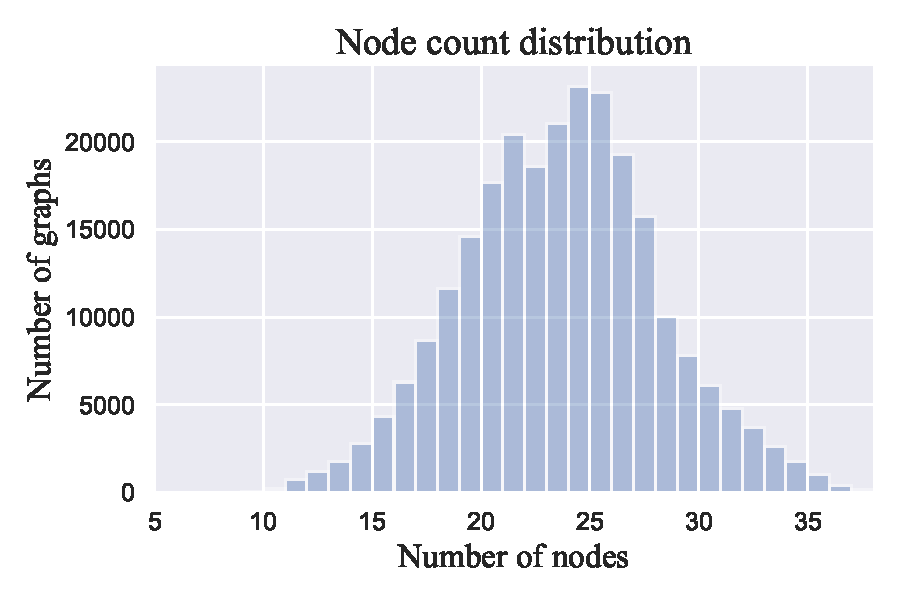
\includegraphics[width=\linewidth]{figures/experiments_figures/dataset_figures/zinc250k/zinc250k_node_distribution.pdf}
       \caption{Zinc250k: Node distribution}
    \end{subfigure}
    \hfill
    \begin{subfigure}{0.49\textwidth}
       \centering
       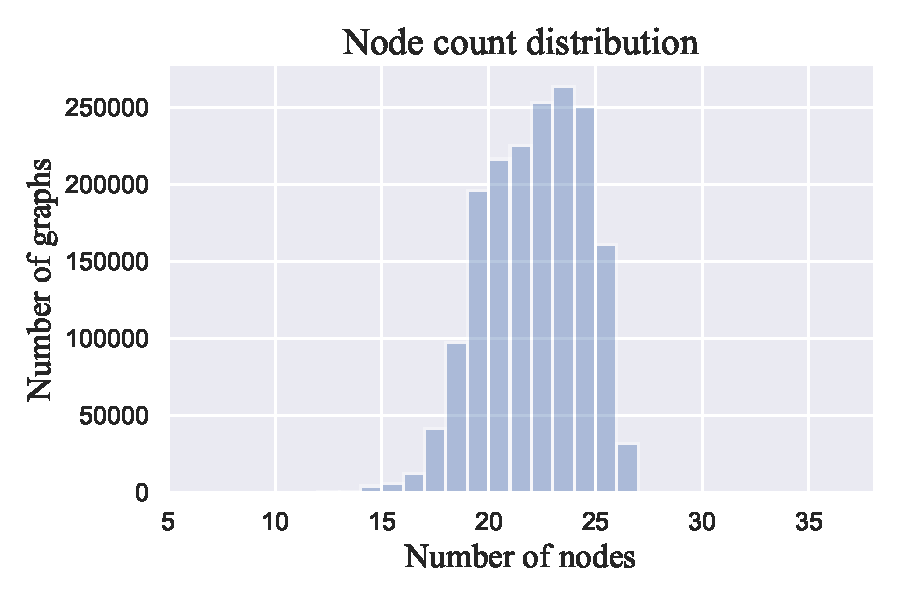
\includegraphics[width=\linewidth]{figures/experiments_figures/dataset_figures/moses/moses_node_distribution.pdf}
       \caption{Moses: Node distribution}
    \end{subfigure}
    \begin{subfigure}{0.49\textwidth}
       \centering
       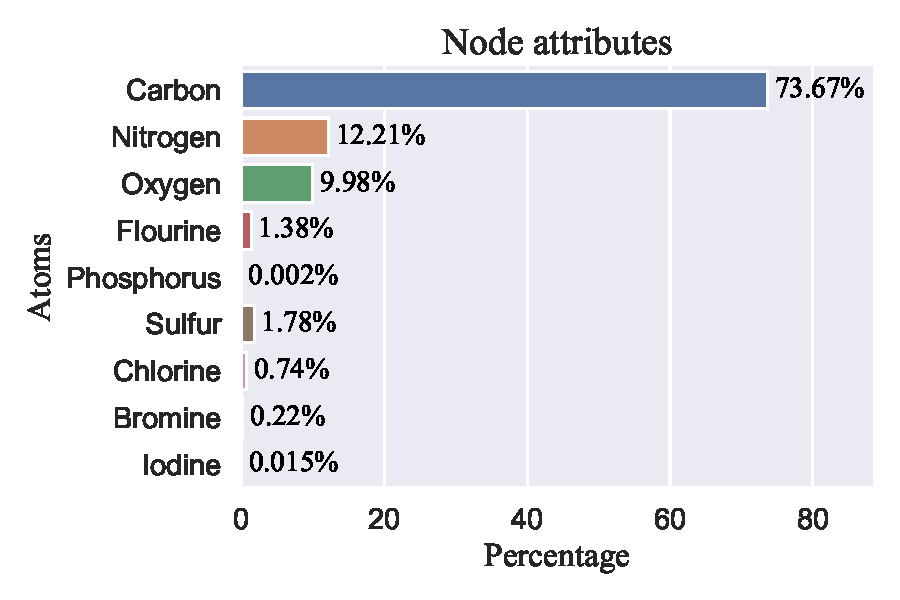
\includegraphics[width=\linewidth]{figures/experiments_figures/dataset_figures/zinc250k/zinc250k_node_attributes.pdf}
       \caption{Zinc250k: Node attributes}
    \end{subfigure}
    \hfill
    \begin{subfigure}{0.49\textwidth}
       \centering
       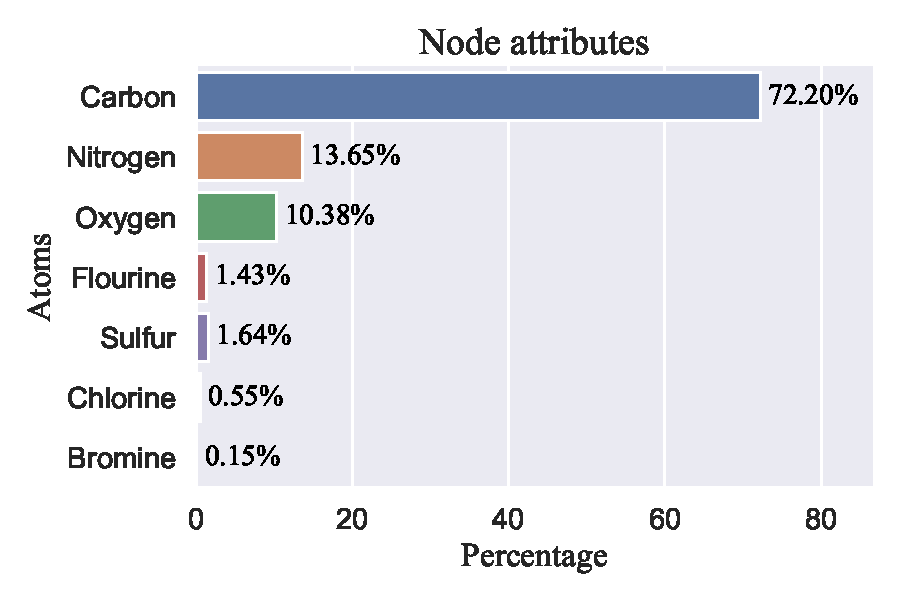
\includegraphics[width=\linewidth]{figures/experiments_figures/dataset_figures/moses/moses_node_attributes.pdf}
       \caption{Moses: Node attributes}
    \end{subfigure}
    \begin{subfigure}{0.49\textwidth}
       \centering
       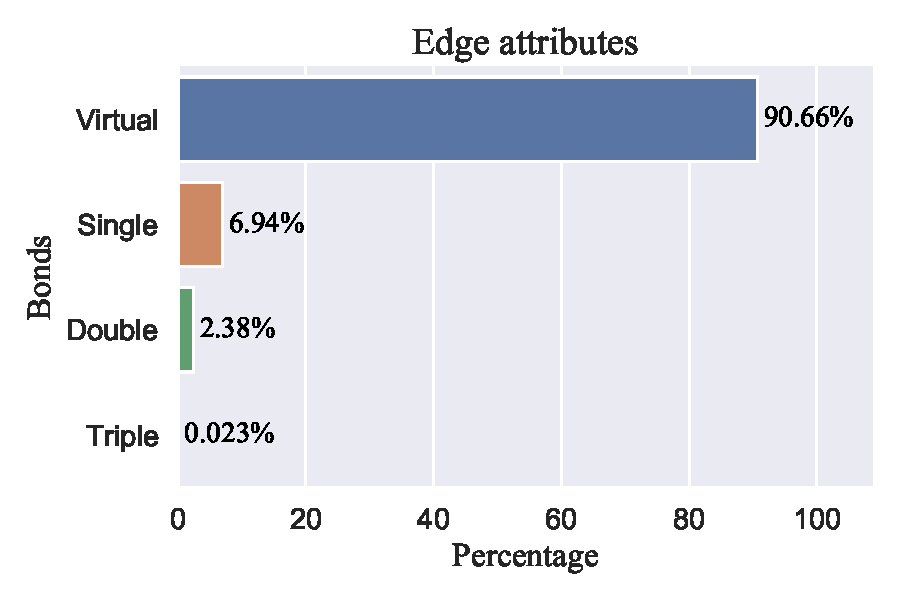
\includegraphics[width=\linewidth]{figures/experiments_figures/dataset_figures/zinc250k/zinc250k_edge_attributes.pdf}
       \caption{Zinc250k: Edge attributes}
    \end{subfigure}
    \hfill
    \begin{subfigure}{0.49\textwidth}
       \centering
       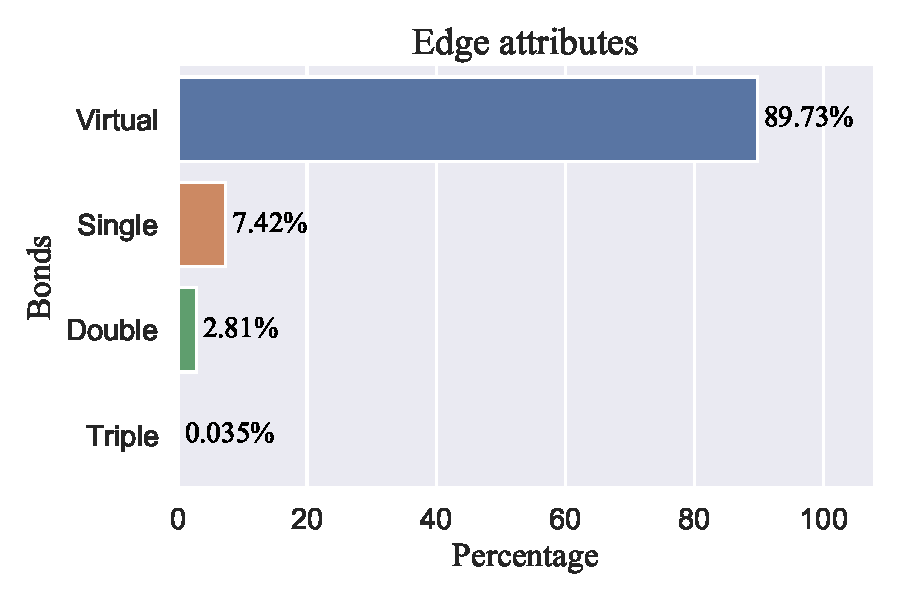
\includegraphics[width=\linewidth]{figures/experiments_figures/dataset_figures/moses/moses_edge_attributes.pdf}
       \caption{Moses: Edge attributes}
    \end{subfigure}
    \caption[Dataset statistic of Zinc250k and Moses]{Dataset statistic of Zinc250k and Moses. (a,b) The node count distribution represents the number of nodes per graph in the dataset. (c,d) The plot shows the frequency of an arbitrary node having a specific categorical node attribute, i.e. atom type. (e,f) Similar to the node attributes, we visualize here the percentage of edges being single, double or triple bonds. The category "virtual" represent the cases where there is no connection/bond between two atoms. }
    \label{fig:appendix_molecule_generation_dataset_statistics}
\end{figure}
\newpage


\subsection{Language modeling}

\paragraph{Dataset details} The three datasets we use for language modeling are the Penn Treebank \cite{PennTreeBank}, text8 \cite{text8} and Wikitext103 \cite{Wikitext}. The Penn Treebank with a preprocessing of \citet{mikolov2012subword} consists of approximately 5M characters and has a vocabulary size of $K=51$. We follow the setup of \citet{SemiDiscreteNFSequence} and split the dataset into sentences of a maximum length of 288. Furthermore, instead of an end-of-sentence token, the length is passed to the model and encoded by an external discrete prior which is created based on the sentence lengths in the training dataset.

Text8 contains about 100M characters and has a vocabulary size of $K=27$. We again follow the preprocessing of \citet{mikolov2012subword} and split the dataset into 90M characters for training, and 5M characters each for validation and testing. We train and test the models on a sequence length of 256.

In contrast to the previous two datasets, we use Wikitext103 as a word-level language dataset. First, we create a vocabulary and limit it to the most frequent 10,000 words in the training corpus. We thereby use pre-trained Glove \cite{Glove} embeddings to represent the words in the baseline LSTM networks and to determine the logistic mixture parameters in the encoding distribution of Categorical Normalizing Flows. Due to this calculation of the mixture parameters, we use a small linear network as a decoder. The linear network consists of three linear layers of hidden size 512 with GELU \cite{GELU} activation and output size of 10,000 (the vocabulary size). Similarly to text8, we train and test the models on an input sequence length of 256.

\paragraph{Hyperparameter details} The hyperparameters for the language modeling experiments are summarized in Table~\ref{tab:appendix_hyperparameters_language_modeling}. We apply the same hyperparameters for the flow and baseline if applicable. The best latent dimensionality for character-level has been shown to be 3, although larger dimensionality showed to gain similar performance. For the word-level dataset, it is beneficial to increase the latent dimensionality to 10. However, note that 10 is still significantly smaller than the Glove vector size of 300. As Penn Treebank has a limited training dataset on which LSTM networks easily overfit, we use a dropout \cite{Dropout} of 0.3 throughout the models and dropout an input token with a chance of 0.1. The other datasets seemed to benefit slightly by a small input dropout to prevent overfitting at later stages of the training.

\begin{table}[ht!]
    \centering
    \caption[Hyperparameter overview for the language modeling experiments]{Hyperparameter overview for the language modeling experiments presented in Table~\ref{tab:result_table_token_level}}
    \label{tab:appendix_hyperparameters_language_modeling}
    \renewcommand{\arraystretch}{1.2}
    \begin{tabular}{lccc}
        \toprule
        \textbf{Hyperparameters} & \textbf{Penn Treebank} & \textbf{text8} & \textbf{Wikitext103}\\
        \midrule
        (Max) Sequence length & 288 & 256 & 256 \\
        Latent dimension & \{2, \underline{3}, 4\} & \{2, \underline{3}, 4\} & \{8, \underline{10}, 12\}\\
        \#Coupling layers & 1 & 1 & 1 \\
        Coupling network & LSTM & LSTM & LSTM \\
        - Number of layers & 1 & 2 & 2 \\
        - Hidden size & 1024 & 1024 & 1024 \\
        - Dropout & \{0.0, \underline{0.3}\} & 0.0 & 0.0 \\
        - Input dropout & \{0.0, 0.05, \underline{0.1}, 0.2\} & \{0.0, \underline{0.05}, 0.1\} & \{0.0, \underline{0.05}, 0.1\} \\
        \#Mixtures & 51 & 27 & 64 \\
        Batch size & 128 & 128 & 128\\
        Training iterations & 100k & 150k & 150k\\
        Optimizer & RAdam & RAdam & RAdam\\
        Learning rate & 7.5e-4 & 7.5e-4 & 7.5e-4 \\
        \bottomrule
    \end{tabular}
\end{table}
